\documentclass{spec}

\newcommand{\syntax}[1]{
	\subsubsection*{Syntax}
	\begin{tabbing}
	\hspace{2cm}\=\\[-16pt]
	#1
	\end{tabbing}
}
\gdef\compat{}
\newcommand{\mustuse}[1]{\must\ be ignored if no ASS3 Extension declaration was used%
\gappto{\compat}{\hspace{9pt} #1 & \textbf{required}\\[3pt]}}
\newcommand{\mayuse}[1]{\may\ be used in non-ASS3 files, but a warning \should\ be emitted.%
\gappto{\compat}{\hspace{9pt} #1 & optional\\[3pt]}}
\newcommand{\secspec}[1]{Section:\>\texttt{#1}}
\newcommand{\secspecs}[2]{Sections:\>\texttt{#1}, \texttt{#2}}
\definecolor{prelim}{rgb}{0,0.3,.6}

\begin{document}
\title{Advanced Sub Station Alpha 3}
\subtitle{{\color{prelim}preliminary specification, subject to change}}
\author{David Lamparter \texttt{<equinox@diac24.net>}}
\contrib{Rodrigo Braz Monteiro \texttt{<amz@>}\\
Niels Martin Hansen \texttt{<jfs@>}}
\spectitle

\section{Abstract}
This document outlines an extension of the \emph{Sub Station Alpha}\cite{SSA}
subtitle data format. It is based on earlier extensions, particularly
ASS (\emph{Advanced SSA}, \cite{ASS}) and ASS2\cite{ASS2}. Since the
specifications for these formats already are pretty vague, the possibilities
for this specification are rather limited.

As SSA, ASS and ASS2 were basically specified by the set of features
implemented by the Sub Station Alpha and VSFilter\cite{VSFilter} applications,
respectively, this specification is largely based on the set of features
implemented by asa\cite{asa}.

A significant amount of features specified herein are based on the
AS5\cite{AS5} specification currently under development. This specification
backports compatible extensions from there.

\subsection{Usage context}
This document makes no incompatible modifications to existing structures,
making it possible to use the extensions defined herein with both ASS and
ASS2 format files. Theoretically, usage with SSA format files is possible
as well; this is by specification forbidden.

ASS3 files are recognised by an \texttt{Extension:~ASS3} declaration in the
\texttt{[Script Info]} header (cf. \ref{Extensions}). The \texttt{ScriptType}
header can be either \texttt{v4.00+} or \texttt{v4.00++}, selecting the
fields used on style and dialogue lines.

\subsection{Conventions}
This document uses the following keywords as specified in RFC2119\cite{2119}:\\
\may, \should, \shouldnot, \must, \mustnot.

Examples in this specification use incomplete \texttt{Format:} lines.
\textbf{This serves illustration purposes only. This specification does \emph{not}
specify usage of non-standard \texttt{Format:} lines, and scripts \mustnot\ use them.}

\section{Overall modifications}
\subsection{ASS Streaming}
The Matroska project\cite{mkv} specifies a format for packetising ASS data.
The format of a data packet is defined as follows:

\begin{verbatim}
[ReadOrder],[Layer],Style,Name,MarginL,MarginR,MarginV,Effect,Text
\end{verbatim}

Start/end timestamps are passed down from the container format. Any non-event
data (script header, styles) is included in the codec-private header.

The ASS3 specification includes this packetisation and clarifies the following
points:
\begin{itemize}
\item \texttt{Format:} lines do not affect the data packet format.
The data packet format is fixed as documented above. Also, while ASS2 \may\ 
be used in the header part, data packets do not use \texttt{MarginT} and
\texttt{MarginB}.
\item \texttt{Dialogue:} lines \mustnot\ be included in the codec-private
header. Renderers \should\ process them anyway, in spite of compatibility.
\item data packets \mustnot\ contain comments (indicated with \verb!;! or
\verb;!;)
\end{itemize}

\subsection{HTML colours}
\syntax{\mustuse{HTML colours}}

\begin{verbatim}
\[1234]c#[AA]RRGGBB
\[1234]a#AA
\alpha#AA
Style: #[AA]RRGGBB
\end{verbatim}

\subsubsection*{Interpretation}
In addition to the existing raw decimal and \verb!&HBBGGRR[AA]! formats,
\verb!#[AA]RRGGBB! colour specifications are allowed in any
place the former two appear.

Regarding alpha values, colour specifications are treated differently
based upon their digit length. If the colour is specified using six
hexadecimal digits, the alpha value is not affected or defaults to zero
for styles. If the colour is specified using eight digits, the alpha
value is set using the first two digits. Any other number of digits
is an invalid use.

Note that the ``HTML'' title does not imply availability of colour names
like ``red'' or ``black''.

\subsubsection*{Compatibility}
As long as ASS3 does not gain widespread software support, this syntax
\shouldnot\ be used for subtitle distribution. Use cases include
hardsubbing and pre-distribution circulation (implying conversion to
standard syntax before distribution).

\subsubsection*{Examples}
\begin{verbatim}
Format: PrimaryColour
Style: #00FF0000

Format: Text
Dialogue: {\1c#00FF00\alpha#CC}
Dialogue: {\3c#4400FF00}
\end{verbatim}

\section{New commands}
\subsection{\texttt{StyleEx:}}
\syntax{
	\secspecs{[V4+ Styles]}{[V4++ Styles]}\\
	\mustuse{StyleEx}
}

\begin{verbatim}
StyleEx: Name, [Parent], [Override codes]
\end{verbatim}

\subsubsection*{Interpretation}
This command defines a new style, named by the first and only required
parameter. The style is inserted into the same namespace as used by the
\verb!Style:! command.

Depending on the other parameters, the style is defined as follows:
\begin{itemize}
\item if the \emph{Parent} parameter is present, the style named by it is
copied. Otherwise, a renderer-dependent default style is loaded.
\item any override codes present are executed on top of the previously
loaded Style. Override codes which cannot be resolved immediately are
retained for execution upon reference (e.g. \verb!\t!).
\end{itemize}

\subsubsection*{Compatibility}
For renderers not supporting \verb!StyleEx!, standard \verb!Style:! lines
\should\ be added, using the same style name. Renderers implementing
\verb!StyleEx! \must\ therefore give higher priority to this command,
making it possible to override the compatibility definitions.

\subsubsection*{Examples}
\begin{verbatim}
Use: ass3.styleex

[V4+ Styles]
Format: Name, Fontname, Fontsize
Style: A, Arial, 16
StyleEx: B, A, \fnTahoma
StyleEx: C, B, \t(\fs24)
\end{verbatim}

\newpage
\subsection{\texttt{Extensions:}}
\label{Extensions}
\syntax{\secspec{[Script Info]}}

\begin{verbatim}
Extensions: [Token[,Token[,...]]]
Extensions: ASS3
\end{verbatim}

\subsubsection*{Interpretation}
This script header key defines the extension set used by the script.
The comma-separated list specifies the extensions to activate and
modifies renderer behaviour.

The ASS3 specification defines only one token, ``\texttt{ASS3}'',
which enables the features outlined in this document. Unknown values
\must\ be ignored.

\section{Modifications to existing commands}
\subsection{\texttt{Dialogue:} with arbitrary precision timestamps}
\syntax{
	\secspec{[Events]}\\
	\mayuse{arbitrary precision timestamps}
}

\subsubsection*{Interpretation}
By legacy from SSA, timestamps in ASS files have centisecond precision.
This extension lifts this limitation by allowing more than two digits
after the separating dot. Together with the second part, this can be
interpreted as plain decimal notation.

However, for compatibility reasons, scripts \mustnot\ use less than two
digits.

\subsubsection*{Compatibility}
Since timestamps are usually processed by the producers of the script
(either by hardsubbing or by converting into container timestamps for
softsubs), this extension can be used as available.
 
\subsubsection*{Example}
\begin{verbatim}
Format: Start
Dialogue: 0:00:01.100
Dialogue: 0:00:03.12815
\end{verbatim}

\subsection{\texttt{Dialogue:} \texttt{\{* \}} for in-line comments}
\syntax{
	\secspec{[Events]}\\
	\mustuse{in-line comments}
}
\begin{verbatim}
Format: Text
Dialogue: ...{*...}...
\end{verbatim}

\subsubsection*{Interpretation}

Existing SSA/ASS versions notably lack a possibility to introduce an
in-line comment. ASS3 defines \texttt{\{*} to start an in-line comment,
which spans all text until the next \texttt{\}} or until the end of the line.

Escape sequences and override codes \mustnot\ be honoured inside comments
declared this way. This implies that override sections can be commented out by
adding a \texttt{*} in front, and it also means that \texttt{\}} cannot
be used inside these comments.

There \mustnot\ be any white-space between the opening curly brace and the
star.

Together with the introduction of this sequence, (ab)using override blocks
for comments is declared invalid and \mustnot\ be used anymore. Comments in
ASS3 scripts \must\ be added using either \texttt{\{*} syntax or via the
\texttt{Comment:} command.

{\footnotesize
\textbf{Background:} A rather large number of subtitle authors appears to be
using the space between curly braces (\texttt{\{\}}) for in-line comments.
Although improbable, this can lead to problems with future extensions
as well as with broken or buggy processing software.
}

\subsubsection*{Examples}
\begin{verbatim}
Format: Text
Dialogue: This is {*not}visible.
Dialogue: And this has {*\fs100}the same font size everywhere.
\end{verbatim}

\section{New override codes}
\subsection{\oc{fax}, \oc{fay}}
\syntax{\mayuse{\oc{fax}, \oc{fay}}}
\begin{verbatim}
\fax<decimal>
\fay<decimal>
\end{verbatim}

\subsubsection*{Interpretation}
The \oc{fax} and \oc{fay} commands introduce a translation to be applied to
glyph outlines. They are given by the following formulae:

\oc{fax}:
$$x' = x + \lambda y$$

\oc{fay}:
$$y' = y + \lambda x$$

Where $\lambda$ represents the parameter value (which can be any decimal
value). $x$ and $y$ iterate over glyph outline coordinates, relative to
\oc{org}. The axes point rightwards and upwards, respectively.

If both \oc{fax} and \oc{fay} are used, the formulae are calculated
simultaneously, not affecting each other's input. They can be represented
by the following matrix:

$$P' = \begin{pmatrix}
1 & \lambda_{\text{fax}} \\
\lambda_{\text{fay}} & 1
\end{pmatrix} \cdot P\;, \quad P = \begin{pmatrix}x \\ y\end{pmatrix}$$

The $\lambda$ value for \oc{fax} / \oc{fay} not given is $0$. The translation
does not affect layout, collision detection or baseline advancement.

\subsubsection*{Examples}
\begin{verbatim}
Format: Text
Dialogue: {\fax-0.1}This text will appear slightly italic.
Dialogue: {\fay1}This text runs 45 degrees downwards.
\end{verbatim}

\subsubsection*{Compatibility}
These two overrides have roots dating back to TextSub 2.23, and
recently (Spring 2007) VSFilter builds are commonly seen with
patches applied. However, portable rendering behaviour cannot
be guaranteed. These overrides \may\ be used with due care.

\subsubsection*{Reference rendering}
\begin{minipage}{6.5cm}
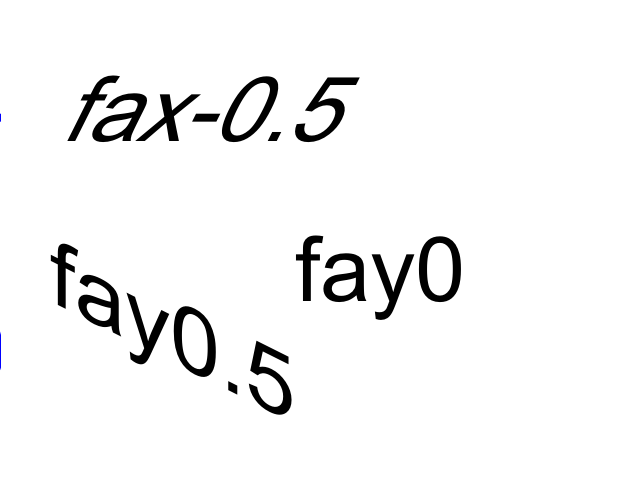
\includegraphics[height=4cm]{ass3_faxfay.png}\\
\textsf{\scriptsize Rendering output: asa git \texttt{f5a1c889}...}
\end{minipage}
\begin{minipage}{6.5cm}
{\footnotesize
\begin{verbatim}
PlayResX: 640
PlayResY: 480
Dialogue: {\an1\pos(50,160)\fax-0.5}fax-0.5
Dialogue: {\an1\pos(50,320)\fay0.5}fay0.5{\fay0}fay0
\end{verbatim}
\emph{Script shortened to fit}
}
\end{minipage}

\subsection{\todo \oc{fsc}}
\ann{\oc{fscx}+\oc{fscy}, is this in any spec yet?}

\subsection{\todo \oc{fa}}
\ann{\oc{fa}: font alternatives. use like: \oc{fnFirstFontToTry}\oc{fa(Fallback1,Fallback2)}}

\ann{If \oc{fn} is not found, emit a warning and try \oc{fa} in order. If \oc{fn} is missing a glyph,
do the same (warning only in debug mode or something).}

\ann{Separate from \oc{fn} for compatibility.}

\section{Modifications to existing override codes}
\subsection{\todo \oc{t} with \oc{pos}, \oc{org}}
\syntax{\mustuse{animated \oc{pos}, \oc{org}}}

\subsection{\oc{pos}, \oc{org} with decimal coordinates}
\syntax{\mayuse{decimal \oc{pos}}}

\subsubsection*{Interpretation}
Traditionally, increasing SSA coordinate resolution to sub-pixel
resolution involved increasing \texttt{PlayRes}. This extension
allows decimal coordinates, removing the need for increasing
\texttt{PlayRes}.

The \oc{move} override \should\ also be implemented using
decimal coordinates. However, replacing \oc{move} by
\oc{t(\oc{pos})} is recommended for ASS3 scripts.

\subsubsection*{Compatibility}
Compatibility of this extension relies on software cutting off
the decimal part and therefore is rather well.
 
\subsubsection*{Example}
\begin{verbatim}
Format: Text
Dialogue: {\pos(271.82818,314.1592)}
\end{verbatim}

\subsection{\todo \oc{k*} with arbitrary precision timings}

\section{Other notes regarding existing override codes}
\subsection{\todo Multiple \oc{t} per line}
\ann{(just clarifications, also compatibility note about ordering with VSFilter)}

\subsection{\oc{r0} deprecation}

The \oc{r0} command in particular--and any use of zero or unrecognisable
parameters in general--to reset a style override to its style default is
declared deprecated by ASS3 and \mustnot\ be used in ASS3 scripts.

To reset a styling option to its style default, scripts \may\ use the
corresponding override tag without any argument. Any parameter value
\must\ be evaluated by processing software in its appropriate context.

\subsection{\texttt{+/-parameter} compatibility}

For some override tags, VSFilter supports an undocumented relative value
syntax, as in \oc{fs+5}. This extension is neither documented, nor well-known,
nor compatible with other renderers. Even worse, it is unclear which tags
it works on, since for example \oc{fscx} may pretty well take a negative
argument.

This syntax is explicitly not part of ASS3 and \should\ be avoided.

\appendix
\section{Appendix}
\subsection{\texttt{Extension:} requirements}

\begin{tabular}{ll}
Extension & \texttt{Extension:~ASS3}\\[6pt]
\compat
\end{tabular}

\subsection{\todo Sample script}

\texttt{\footnotesize
Add me! Mommy! Add me!
}

\addcontentsline{toc}{section}{References}
\begin{thebibliography}{1}
\bibitem{SSA} Kotus, Sub Station Alpha. Website, 1997-2003.\\
\url{http://web.archive.org/web/*/http://www.eswat.demon.co.uk/substation.html}

\bibitem{ASS} \#Anime-Fansubs, Advanced Sub Station Alpha.\\
\url{http://www.anime-fansubs.org}\\
\url{http://moodub.free.fr/video/ass-specs.doc}

\bibitem{ASS2} Gabest, Advanced Sub Station Alpha 2. SVN, 2005.\\
\url{http://svn.sourceforge.net/viewcvs.cgi/guliverkli/trunk/guliverkli/src/subtitles/STS.cpp?r1=423&r2=453}

\bibitem{VSFilter} Gabest, VSFilter. Application, 2003-2007.\\
\url{http://sourceforge.net/projects/guliverkli/}

\bibitem{asa} equinox, asa. Application, 2004-2007.\\
\url{http://asa.diac24.net/}

\bibitem{AS5} ArchMage ZeratuL et al., AS5. Draft, 2006-2007.\\
\url{http://asa.diac24.net/AS5}

\bibitem{2119} S. Bradner, Key words for use in RFCs to Indicate Requirement Levels. RFC, 1997.\\
\url{http://www.ietf.org/rfc/rfc2119.txt}

\bibitem{mkv} The Matroska project.\\
\url{http://www.matroska.org/}

\end{thebibliography}
\end{document}
